\chapter{Estabilidad de los Amplificadores Realimentados}

\hspace{10pt} \textbf{Ejercicio 1}: Un amplificador tiene una ganancia a lazo
abierto a frecuencias medias $a_o= 200$ y su función transferencia,
a lazo abierto, tiene tres polos en: 1 MHz, 2 MHz y 20 MHz. a)
Construir el diagrama de Bode para el amplificador sin realimentar.
b) Calcular el valor de $T_o$ que causa inestabilidad. c)  Calcular
los valores de f (factor de realimentación suponiéndolo resistivo
puro) necesarios para obtener un margen de fase de 65°, 40° y 20°
respectivamente. d)  Graficar para los tres casos del inciso
anterior el módulo y la fase de la ganancia realimentada $|A_f(w)|$.
e) Calcular los sobrepicos de la respuesta de la ganancia a lazo
cerrado, por encima del valor correspondiente a frecuencias medias,
en las proximidades de la frecuencia donde $|T(jw)|=1$.

\textbf{Ejercicio 2}: Repetir el ejercicio anterior, pero en el caso
en que las frecuencias correspondientes a los polos del amplificador
sin realimentar sean: 1 MHz, 2 MHz y 4 MHz. Calcular el $T_o$
crítico empleando el criterio de Routh-Hurwitz.

\textbf{Ejercicio 3}: Un amplificador tiene una ganancia de baja
frecuencia $a_o= 5000$ y su función transferencia posee tres polos
en 0,3 MHz, 2 MHz y 25 MHz. a)  Calcule la frecuencia del polo
dominante requerida para dar la compensación por ganancia unitaria
de este amplificador con un margen de fase de 45°. b)  Compense de
igual manera que en el inciso anterior utilizando la técnica de
correr el primer polo, indicando la nueva ubicación de dicho primer
polo.

\textbf{Ejercicio 4}:  El amplificador de la figura \ref{eje4} tiene
dos polos. Suponga que la ganancia de lazo ($T_o$) puede ser
cambiada, sin variar los parámetros del amplificador sin
realimentar. Dibuje el lugar de raíces cuando $f_o$ varía entre 0 y
0,01, con y sin $C_f$, con los valores dados de $R_e$ y $R_f$.
Dibuje en cada caso la gráfica de ganancia.

\begin{figure}[h]
	\centering
	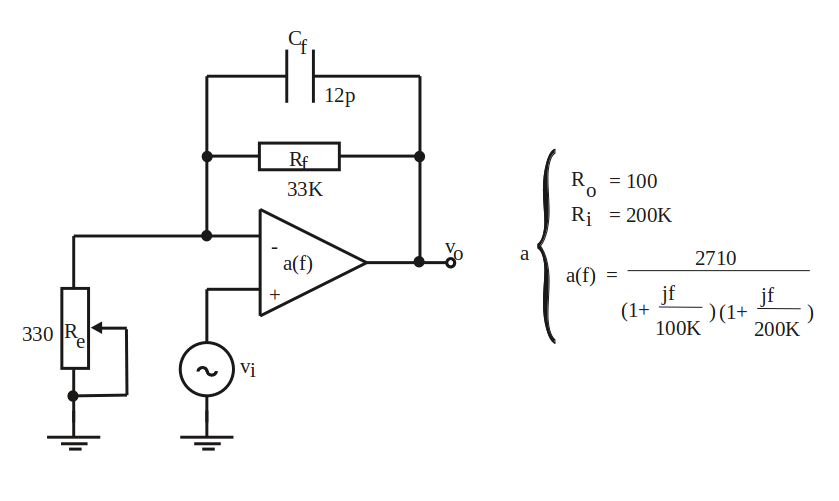
\includegraphics[width=0.8\linewidth]{figuras/estab4.png}\\
	\caption{Ejercicio 4.}\label{eje4}
\end{figure}

\textbf{Ejercicio 5}: En el circuito de la figura \ref{eje5} suponga
que el amplificador de tensión sin realimentar $a(jf)$ tiene un $a_o
= 43000$ y que posee tres polos en 10 KHz, 30 KHz y 300 KHz . a)
Hallar el valor de $R_f$ para obtener una ganancia a frecuencias
medias del sistema realimentado $\frac{\displaystyle
	v_o}{\displaystyle v_1}=-1000$. b) Trazar el lugar de raíces del
mismo para el caso de $C_f=0$. Utilizando el criterio de
Routh-Hurwitz, determinar si en este caso el amplificador es
estable. c)  Calcular el sobrepico de la ganancia y la respuesta al
escalón en forma aproximada, en las condiciones del punto a). d)
Calcular $C_f$ de manera de compensar introduciendo un cero en la
frecuencia a la que se produce el sobrepico de la ganancia (explicar
este método de compensación). Graficar la nueva curva de
transferencia del sistema realimentado.

\begin{figure}[h]
	\centering
	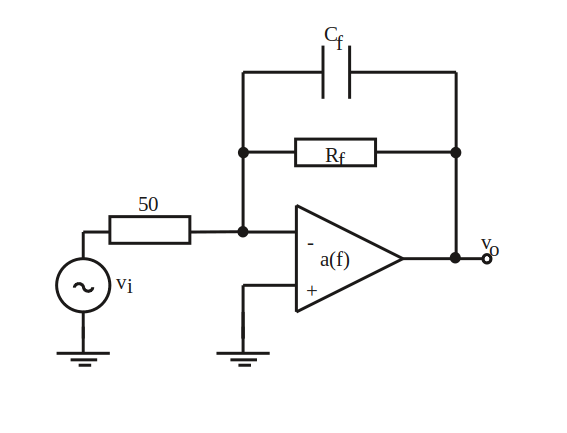
\includegraphics[width=0.8\linewidth]{figuras/estab5.png}\\
	\caption{Ejercicio 5.}\label{eje5}
\end{figure}

\textbf{Ejercicio 6}:   Dado el circuito de la figura \ref{eje6},
hallar por simulación (y luego verificar por cálculo): a)  El
diagrama de Bode del amplificador operacional $\mu a741$ a lazo
abierto. Obtener la ganancia a frecuencias bajas y estimar la
ubicación de los polos a lazo abierto. b)  Obtener el diagrama de
Bode de amplitud y fase y la respuesta al escalón del amplificador
realimentado, compararlo con el resultado teórico. c)  Cargar el
circuito con una carga capacitiva $Z_L$ que sea una capacitor de 0,1
$\mu F$ en serie con una resistencia $0 < R_L < 30$  . Sacar
conclusiones.

\begin{figure}[h]
	\centering
	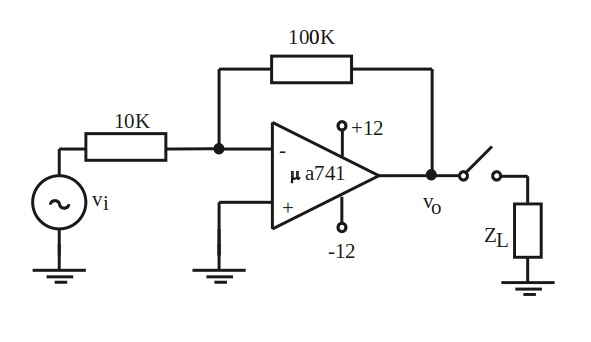
\includegraphics[width=0.8\linewidth]{figuras/estab6.png}\\
	\caption{Ejercicio 6.}\label{eje6}
\end{figure}

\textbf{Ejercicio 7}: Un sistema realimentado tiene una ganancia de
lazo que responde a:

\begin{equation}
	T(s)=T_o \frac{\displaystyle \left (1+\frac{\displaystyle s}{\displaystyle 100}\right )^2}{\displaystyle \left (1+\frac{\displaystyle s}{\displaystyle 1}\right )^3}
	\nonumber
\end{equation}
, analizar la estabilidad del sistema utilizando lugar de raíces,
Routh-Hurwitz y Bode.


\textbf{Ejercicio 8}:   Dado el circuito de la figura \ref{eje8}, a)
hallar el valor de $R_x$ que hace que el margen de fase sea $M \Phi
\approx 0$, b) implementar físicamene la compensación del circuito
para obtener un $M \Phi \approx 45°$ utilizando los métodos de: b1)
polo dominante, b2) corrimiento del primer polo, b3) atraso de fase
y b4) adelanto de fase.


\textbf{Ejercicio 9}: El lugar de raíces de la figura \ref{eje9}
corresponde al circuito realimentado dibujado a la derecha. ¿El
sistema es estable?, ¿cuánto vale la ganancia de lazo a frecuencias
medias $T_o$?.  Graficar las ganancias de tensión con y sin
realimentar en función de la frecuencia (BODE de amplitud). Hallar
el margen de fase y compensar el sistema con un polo dominante de
modo de obtener un margen de fase $M\Phi \geq 45°$. Implementar la
compensación.


\begin{figure}[h]
	\centering
	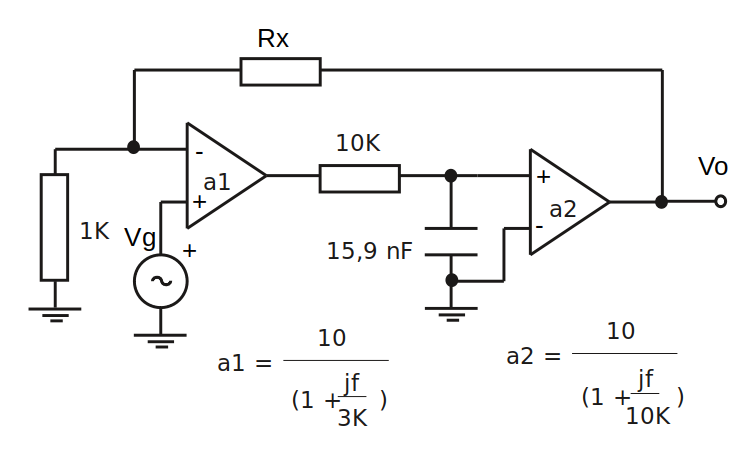
\includegraphics[width=0.8\linewidth]{figuras/estab8.png}\\
	\caption{Ejercicio 8.}\label{eje8}
\end{figure}



\begin{figure}[h]
	\centering
	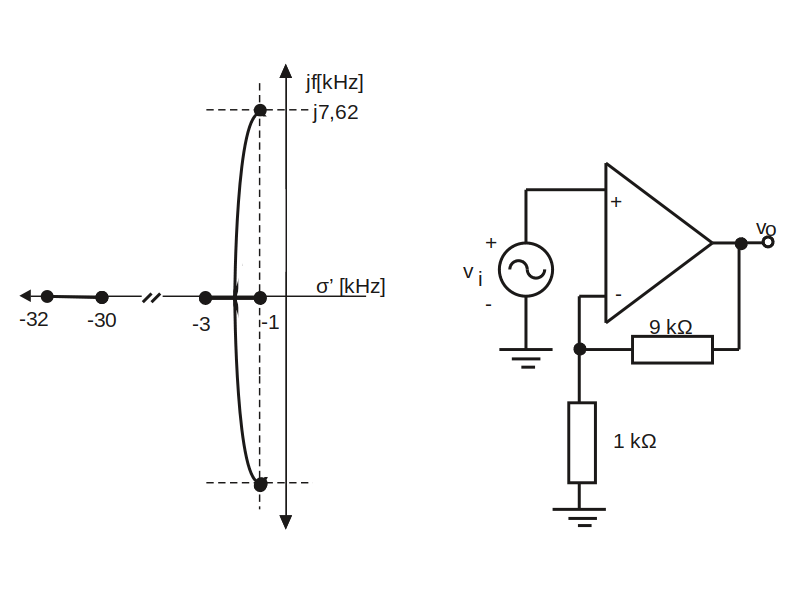
\includegraphics[width=0.8\linewidth]{figuras/estab9.png}\\
	\caption{Ejercicio 9.}\label{eje9}
\end{figure}
